
\documentclass{article} % For LaTeX2e
\usepackage[UTF8,fontset=none,heading=false]{ctex}
\setCJKmainfont[AutoFakeBold=2.5,ItalicFont={Songti SC}]{Songti SC}
\setCJKsansfont[AutoFakeBold=2.5]{Hiragino Sans GB}
\setCJKmonofont[Scale=0.92]{Hiragino Sans GB}
\setmainfont{texgyretermes-regular.otf}[
  BoldFont=texgyretermes-bold.otf,
  ItalicFont=texgyretermes-italic.otf,
  BoldItalicFont=texgyretermes-bolditalic.otf
]
\setsansfont{texgyreheros-regular.otf}[
  BoldFont=texgyreheros-bold.otf,
  ItalicFont=texgyreheros-italic.otf,
  BoldItalicFont=texgyreheros-bolditalic.otf
]
\setmonofont{texgyrecursor-regular.otf}[
  BoldFont=texgyrecursor-bold.otf,
  ItalicFont=texgyrecursor-italic.otf,
  BoldItalicFont=texgyrecursor-bolditalic.otf,
  Scale=MatchLowercase
]
\XeTeXlinebreaklocale "zh"
\XeTeXlinebreakskip = 0pt plus 1pt
\usepackage{iclr2026_conference}

% Optional math commands from https://github.com/goodfeli/dlbook_notation.
\input{math_commands.tex}

\usepackage[font=small,labelfont=bf]{caption}
\usepackage{graphicx,subcaption}
\usepackage{multirow}
\usepackage{hyperref}

\usepackage{algorithm}
\usepackage{algorithmicx}
\usepackage{algpseudocode}
\usepackage{microtype}
\usepackage{booktabs}
\usepackage{arydshln}
\usepackage{float}
\usepackage{bigstrut}
\usepackage[all]{hypcap}
\usepackage{amsmath}
\usepackage{amssymb}
\usepackage{mathtools}
\usepackage{amsthm}
\usepackage{mathrsfs}
\usepackage{nicefrac}
\usepackage{dsfont}
\usepackage{enumitem}
\usepackage{cleveref}
\usepackage[table]{xcolor}
\usepackage{url}            %
\usepackage{amsfonts}       %
\usepackage{wrapfig}
\usepackage{lipsum}
\usepackage{stackengine}
\usepackage{color}
\usepackage{adjustbox}
\usepackage{xspace}
\usepackage{rotating}
\usepackage{makecell}
\usepackage{bbding}
\usepackage{pifont}
\usepackage{wasysym}
\usepackage{tcolorbox}


\renewcommand{\figurename}{图}
\renewcommand{\tablename}{表}
\renewcommand{\refname}{参考文献}
\renewcommand{\appendixname}{附录}
\renewcommand{\figureautorefname}{图}
\renewcommand{\tableautorefname}{表}
\renewcommand{\sectionautorefname}{节}
\renewcommand{\subsectionautorefname}{小节}
\renewenvironment{abstract}{%
  \vskip 0.075in
  \centerline{\large\bfseries 摘要}
  \vspace{0.5ex}
  \begin{quote}
}{%
  \par\end{quote}\vskip 1ex
}

\title{CoAct-1：具备编码动作的计算机使用多智能体系统\\
\large CoAct-1: Computer-using Multi-agent System with Coding Actions}
\iclrfinalcopy

% Authors must not appear in the submitted version. They should be hidden
% as long as the \iclrfinalcopy macro remains commented out below.
% Non-anonymous submissions will be rejected without review.

\author{Linxin Song$^1$\thanks{该工作完成于 Salesforce 实习期间。}, \ Yutong Dai$^2$, Viraj Prabhu$^2$, Jieyu Zhang$^3$, Taiwei Shi$^1$, Li Li$^1$, Junnan Li$^2$\\
\textbf{Silvio Savarese}$^2$, \textbf{Zeyuan Chen}$^2$, \textbf{Jieyu Zhao}$^1$, \textbf{Ran Xu}$^2$, \textbf{Caiming Xiong}$^2$ \\
$^1$南加州大学 \ $^2$Salesforce \ $^3$华盛顿大学  \\
\\
\texttt{代码：} \url{https://github.com/SalesforceAIResearch/CoAct-1}
}

% The \author macro works with any number of authors. There are two commands
% used to separate the names and addresses of multiple authors: \And and \AND.
%
% Using \And between authors leaves it to \LaTeX{} to determine where to break
% the lines. Using \AND forces a linebreak at that point. So, if \LaTeX{}
% puts 3 of 4 authors names on the first line, and the last on the second
% line, try using \AND instead of \And before the third author name.

\newcommand{\fix}{\marginpar{FIX}}
\newcommand{\new}{\marginpar{NEW}}
\newcommand{\ours}{CoAct-1\xspace}
\newcommand\draftcomment[1]{\textbf{#1}}
\newcommand{\lx}[1]{\draftcomment{\textcolor{purple}{[#1]$_{-\text{Linxin}}$}}}
\newcommand{\todo}[1]{\textcolor{red}{\textbf{VP:} #1}}
\newcommand{\yd}[1]{\textcolor{orange}{\textbf{YD:} #1}}
\newcommand{\jz}[1]{\textcolor{blue}{[Jieyu Zhao: #1]}}
\newcommand{\best}[1]{\underline{#1}}

\definecolor{lightblue}{rgb}{0.22, 0.45, 0.70}%
\definecolor{Gray}{gray}{0.95}
\definecolor{Cornsilk}{rgb}{1.0, 0.97, 0.86}

%\iclrfinalcopy % Uncomment for camera-ready version, but NOT for submission.
\begin{document}
\maketitle
\begin{abstract}
通过图形用户界面（GUI）操作计算机的自主智能体，在复杂的长时程任务上往往难以兼顾效率与可靠性。为这类智能体加入规划器虽然能够改善任务分解，但若所有动作仍必须通过 GUI 操作完成，系统依然受制于这种交互方式固有的局限，因而脆弱且低效。本文提出一种更稳健、更灵活的范式：让智能体把编码作为一种增强动作。我们提出 \ours，这是一种将 GUI 控制与直接程序化执行协同结合的新型多智能体系统。\ours 包含一个编排器（Orchestrator），它把子任务动态委派给传统的 GUI 操作员（GUI Operator）或专门的编程员（Programmer）智能体；后者可以编写并执行 Python 或 Bash 脚本。这种混合方法使智能体能够在文件管理、数据处理等任务中绕过低效的 GUI 动作序列，同时在必要时继续使用视觉交互。我们在具有挑战性的 OSWorld 和 WindowsAgentArena 基准上评估该系统；\ours 在 OSWorld 上取得 60.8\% 的成功率，在 WindowsAgentArena 上取得 52.5\% 的成功率，均达到新的最先进水平并显著优于既有方法。此外，该方法显著提升了效率：在 OSWorld 上，完成任务所需的平均步数降至 10.15，而领先 GUI 智能体需要 15 步。结果表明，将编码整合为核心动作，为通用计算机自动化提供了一条能力更强、效率更高且更具可扩展性的路径。
\end{abstract}

\section{引言}
近期关于计算机使用智能体的进展，主要聚焦于通过图形用户界面（GUI）进行操作。由视觉语言（动作）模型驱动的 GUI 智能体~\citep{blip2,gemini2,gemini25,openai2024gpt4ocard, cua2025, qin2025ui, xie2025scalingcomputerusegroundinguser, yang2025gta1guitesttimescaling} 已经展现出完成多类任务的能力，但在长时程规划以及 GUI 元素密集环境中的交互方面仍常常遇到困难。例如，Office 生产力软件中的日常任务往往涉及漫长而复杂的精确 GUI 操作序列：先在含多个工作表的电子表格中定位特定表格，再按复杂条件筛选、复制结果，并将其保存为新的 CSV 文件。类似地，在嵌套目录结构中查找所有图像文件、把它们缩放至指定尺寸、再将整个目录压缩为单个归档文件；若依靠点击、拖拽等 GUI 动作完成，同样既脆弱又低效。在这些场景中，现有智能体经常受到视觉定位歧义（例如混淆外观相似的图标或菜单项）以及长期交互中错误概率累积的影响。一次误点或对某个界面元素的误解，就可能使整个任务偏离轨道。

为应对这些挑战，一条重要研究路线是为 GUI 智能体配备专门的高层规划器。GTA-1~\citep{yang2025gta1guitesttimescaling} 等方法及其他模块化系统~\citep{yang2024aria, xu2024aguvis, agashe2024agent, agashe2025agent}，使用 OpenAI o3~\citep{openAI_o3_o4_mini} 之类的强大语言模型，将用户的高层目标分解为一系列更易处理的子任务。这样的层次化分解通过提供结构化计划，可以改善复杂多步问题上的表现。然而，该范式并未从根本上解决完全依赖 GUI 执行所带来的低效和脆弱性。即使已经完成高层规划，智能体仍需浏览菜单、点击按钮并向字段输入内容；即便某些操作本可通过程序化手段更直接、更可靠地完成，也不例外。因此，系统仍容易受到规划不确定性、视觉感知错误，以及高层规划与底层动作生成之间整合难题的影响。

本文主张并实现一种更灵活、更强大的动作空间。我们提出一种混合方法，把 GUI 操作直观、类人的优势，与通过代码直接同系统交互所具备的精确性、可靠性和效率结合起来。我们提出 \textbf{\ours}（Computer-using Multi-agent System with \textbf{Co}ding \textbf{Act}ions），它由编排器、编程员和 GUI 操作员三个专用智能体组成。高层编排器充当中央规划器，负责分解用户目标并为每个子任务确定合适的动作模态。根据分析结果，它将任务交给两类不同的执行智能体之一：编程员负责为文件管理、数据处理或环境配置等后端操作编写并执行 Python 或 Bash 脚本；基于视觉语言模型（VLM）的 GUI 操作员则负责点击按钮、浏览可视界面等前端动作。通过这种动态委派，\ours 可以在适当时策略性地跳过低效 GUI 序列，改用稳健的单次代码执行，同时仍可针对需要视觉操作的任务利用视觉交互。

实验分析为这种混合设计的优势提供了有力证据。在 OSWorld 和 WindowsAgentArena 基准上，\ours 分别取得 60.76\% 和 52.50\% 的总体成功率，刷新了最先进水平。在 OSWorld 上，这相较 Agent S2.5（55.98\%）等领先基线有显著提升。在程序化控制优势明显的任务类别中，性能增益最为突出。例如，在 Calc（70.21\%）、多应用（47.88\%）和 VS Code（78.26\%）任务中，编程员执行精确脚本的能力，使系统相较最强的纯 GUI 方法获得大幅提升。除提高成功率之外，我们的双模态方法还显著改善了操作效率。通过用简洁代码替代漫长且易错的点击序列，\ours 在 OSWorld 上平均仅需 10.15 步即可解决任务，与 GTA-1 等智能体所需的 15 步形成鲜明对比。这种效率说明，本方法有望为通用计算机自动化铺就一条更稳健、可扩展的路径。

\section{相关工作}
\label{sec:related-work}

\textbf{屏幕解析与视觉定位。} 第一类工作聚焦于直接从像素中感知和定位 GUI 元素，而不依赖 DOM 或无障碍接口。\textit{OmniParser} 学习用于纯视觉理解的屏幕解析基元~\citep{lu2024omniparser}。在定位方面，\textit{SeeClick}（从指令定位目标）、\textit{Aria-UI}（面向 GUI 的指令定位）和 \textit{UGround}（通用 GUI 定位）把语言映射到屏幕上可执行操作的位置~\citep{cheng2024seeclick,yang2024aria,gou2024uground}。\textit{OS-Atlas} 训练一种\emph{基础动作模型}，使其能够泛化到多样化界面~\citep{wu2024atlas}。\textit{ScreenSpot-Pro} 等专门的定位评测，还进一步衡量了专业高分辨率环境中的定位能力~\citep{li2025screenspotpro}。

\textbf{原生端到端 GUI 智能体。}
另一条路线训练在单一模型中统一感知、推理与动作的\emph{原生}智能体。\textit{UI-TARS} 和 \textit{OpenCUA} 是这种方法的代表：它们使用跨应用的统一鼠标/键盘动作空间，而不采用手工设计的控制器~\citep{qin2025ui, wang2025ui, wang2025opencua}。\textit{AGUVIS} 则进一步探索能够跨界面泛化的统一纯视觉 GUI 智能体~\citep{xu2024aguvis}。

\textbf{模块化规划器--定位器智能体。}
第二类研究明确区分\emph{做什么}与\emph{在屏幕何处、如何操作}：语言规划器提出子目标，视觉模型则定位每一步动作。代表性系统包括 \textit{SeeClick} 和 \textit{OS-Atlas}~\citep{cheng2024seeclick,wu2024atlas}。\textit{GTA-1} 通过\emph{测试时扩展}强化这种两阶段范式：采样多个候选动作，再使用多模态大语言模型（MLLM）裁判从中选择，从而提高系统在高分辨率、元素密集 GUI 上的稳健性~\citep{yang2025gta1guitesttimescaling}。\textit{Agent-S / Agent-S2} 与 \textit{AutoGen} 等其他相关开放框架，则为多智能体编排和工具调用提供了可复用基础设施~\citep{agashe2024agent,agashe2025agent, song2025adaptiveinconversationteambuilding, zhang2024offlinetraininglanguagemodel,wu2023autogenenablingnextgenllm, zhang2023ecoassistantusingllmassistant,zhang2025agentcausestaskfailures}。

\textbf{混合智能体框架。}
在纯 GUI 交互之外，一些智能体系统会在运行时动态组合工具和 API 以扩展能力。例如 \textit{UFO-2}~\citep{zhang2025ufo2desktopagentos}、\textit{PyVision}~\citep{zhao2025pyvisionagenticvisiondynamic}、\textit{BeyondBrowsing}~\citep{song2025browsingapibasedwebagents} 和 \textit{ALITA}~\citep{qiu2025alitageneralistagentenabling}。这些系统虽然不局限于 GUI/计算机使用智能体（CUA），但都遵循动态构造并调用工具的原则。

\section{以编码为动作的计算机使用智能体}
\begin{figure}[h]
    \centering
    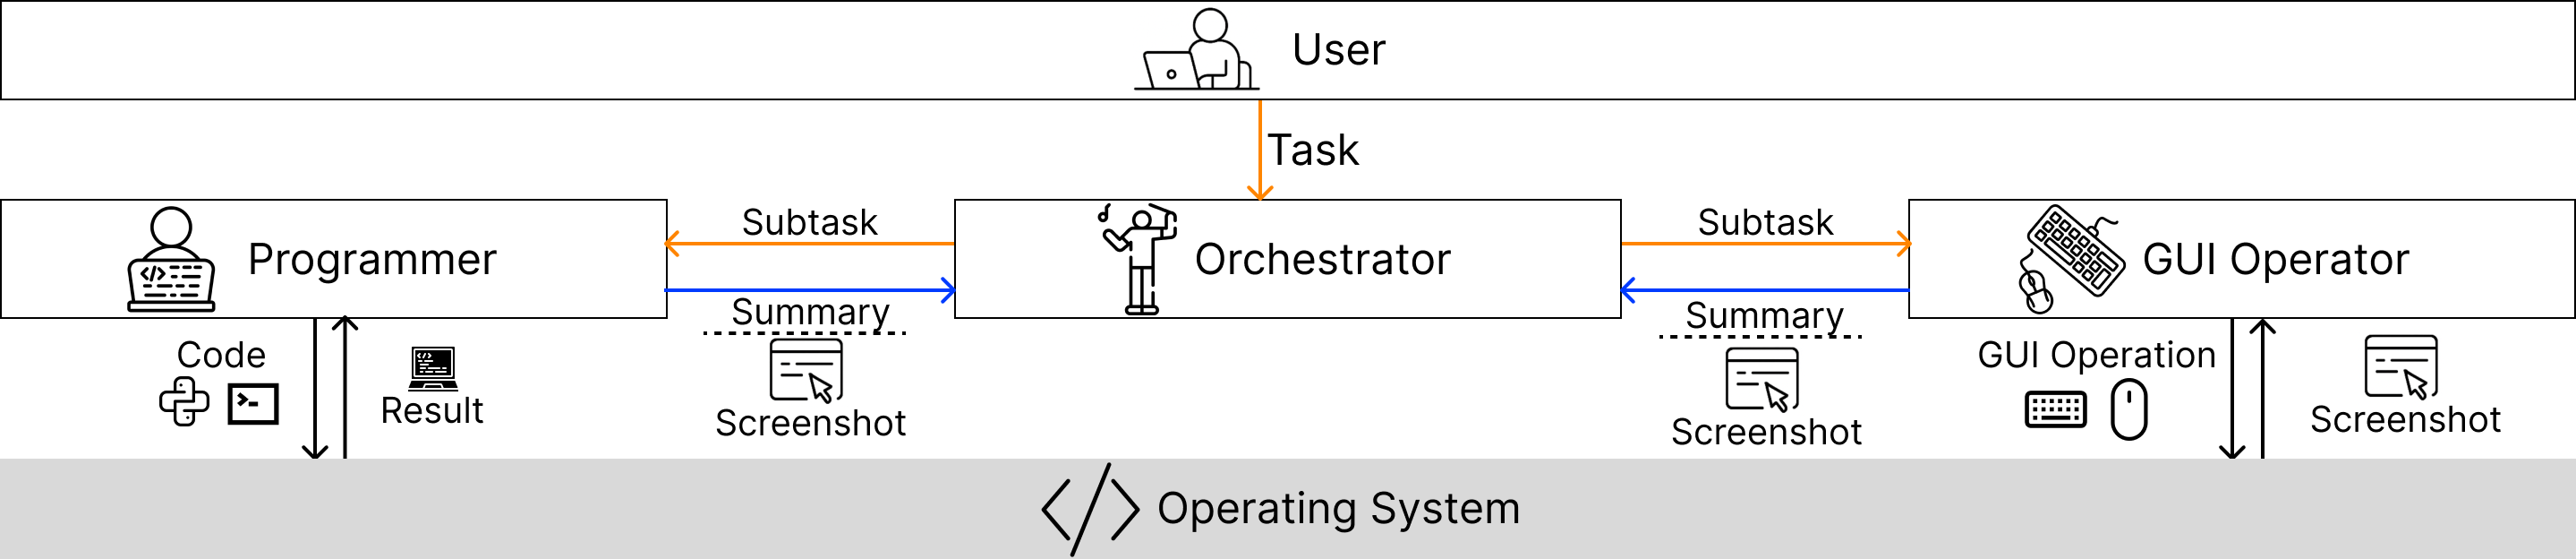
\includegraphics[width=\linewidth]{figures/overall.png}
    \caption{\ours 的多智能体系统设计。系统包括：作为高层规划器、负责分解目标并把子任务委派给合适执行智能体的\textbf{编排器}；通过多轮编码与操作系统交互的\textbf{编程员}；以及利用视觉语言能力执行可视界面动作的 \textbf{GUI 操作员}。}
    \label{fig:overall}
\end{figure}
本文引入一种新的系统交互动作——编码——来替代部分冗余且脆弱的 GUI 动作。不同于为每个应用或网站归纳 API/SDK，我们关注的是让智能体在强语言模型引导下进行自由形式编码，以解决计算机使用问题。
具体而言，我们设计了多智能体系统 \ours，并引入一个能够通过“编码--观测”循环与操作系统交互的新智能体——编程员。编排器充当高层控制器，决定把子任务交给编程员还是 GUI 操作员。整体框架如\autoref{fig:overall}所示。

\subsection{问题定义}
我们把通用计算机控制形式化为一个交互式决策过程。在每个时间步 $t$，智能体观测主要由屏幕截图构成的计算机环境 $o_t\in \gO$，并依据策略 $\pi(a_t \mid H_t, G)$ 采取动作 $a_t\in \gA$。其中，$H_t=(o_1, a_1, \ldots, o_{t-1}, a_{t-1}, o_t)$ 表示历史上下文，$G$ 是用户以自然语言提供的高层目标。当动作空间 $\gA$ 被限制为底层 GUI 操作时，学习有效策略尤其困难。管理嵌套文件、处理电子表格数据等复杂任务，可能需要漫长而繁复的 GUI 动作序列，因而效率低下，并极易发生错误传播：一次误操作就可能使整个任务失败。

为解决这一局限，我们引入整合直接程序化控制的混合动作空间。它在标准 GUI 动作空间基础上扩展而来，记为 $\gA = \gA_{\text{GUI}}\cup \gA_{\text{Code}}$。动作 $a_t\in\gA_{\text{GUI}}$ 表示对图形界面的直接操作（例如鼠标点击、键盘输入）；相较之下，动作 $a_t\in \gA_{\text{Code}}$ 是一段直接与操作系统后端交互的 Python 或 Bash 脚本。这使智能体能够用一个稳健步骤完成文件操作、数据处理等复杂任务，从而有效绕过脆弱低效的 GUI 序列。在 \ours 中，策略 $\pi$ 采用层次化实现：高层编排器充当元策略 $\pi_{\text{orch}}$，分析当前子任务，并将其委派给两个专用执行策略之一——GUI 操作员以 $\pi_{\text{GUI}}$ 实现 $\gA_{\text{GUI}}$ 中的动作，编程员则以 $\pi_{\text{Code}}$ 实现 $\gA_{\text{Code}}$ 中的动作。

\subsection{面向计算机使用的多智能体系统设计}
我们的多智能体系统，是问题定义中层次化策略 $\pi$ 的架构实例。系统包含编排器、编程员和 GUI 操作员三个专用智能体，它们协作生成动作轨迹 $\tau$，以完成用户目标 $G$。每个智能体都建立独立对话来履行各自职责。

\noindent\textbf{编排器。} 编排器实现高层元策略 $\pi_{\text{Orch}}$，依据完整观测历史 $H_t$ 和总体目标 $G$ 负责任务分解与动态规划。编排器不直接同操作系统交互；它的主要职能，是在专用子策略 $\pi_{\text{Code}}$ 和 $\pi_{\text{GUI}}$ 中选择最适合执行当前子任务的一项。子任务完成后，编排器会收到执行过程摘要和新观测 $o_{t+1}$（一张屏幕截图，以及反映当前系统状态的摘要），并以此支持下一步决策。若判断总体目标 $G$ 已经完成，它便输出终止信号。

\noindent\textbf{编程员。} 编程员实现专用策略 $\pi_{\text{Code}}$，负责生成动作 $a_t\in\gA_{\text{Code}}$。收到编排器委派的子任务后，它会与代码解释器展开多轮对话，生成由解释器执行的 Python 或 Bash 脚本。由代码执行结果构成的反馈，使编程员能够反思并改进代码，直至子任务完成。编排器会向编程员提供足够的上下文，例如根据 $H_t$ 推断出的文件路径或窗口信息，从而使其代码生成有明确依据。

\noindent\textbf{GUI 操作员。} GUI 智能体是一个视觉语言动作模型，它实现基于 GUI 的策略 $\pi_{\text{GUI}}$，用于生成动作 $a_t\in\gA_{\text{GUI}}$。与编程员类似，GUI 操作员通过多轮交互循环完成被委派的子任务。在“感知--动作”循环的每一步中，智能体以当前屏幕截图和子任务指令为输入，生成一个 GUI 动作（例如鼠标点击或键盘输入）。GUI 动作解释器在操作系统上执行该动作，操作系统随即提供新的屏幕截图作为观测反馈。GUI 操作员根据新的视觉信息决定后续动作，循环往复，直到子任务完成。

\subsection{工作流与记忆设计}
\begin{figure}[t]
    \centering
    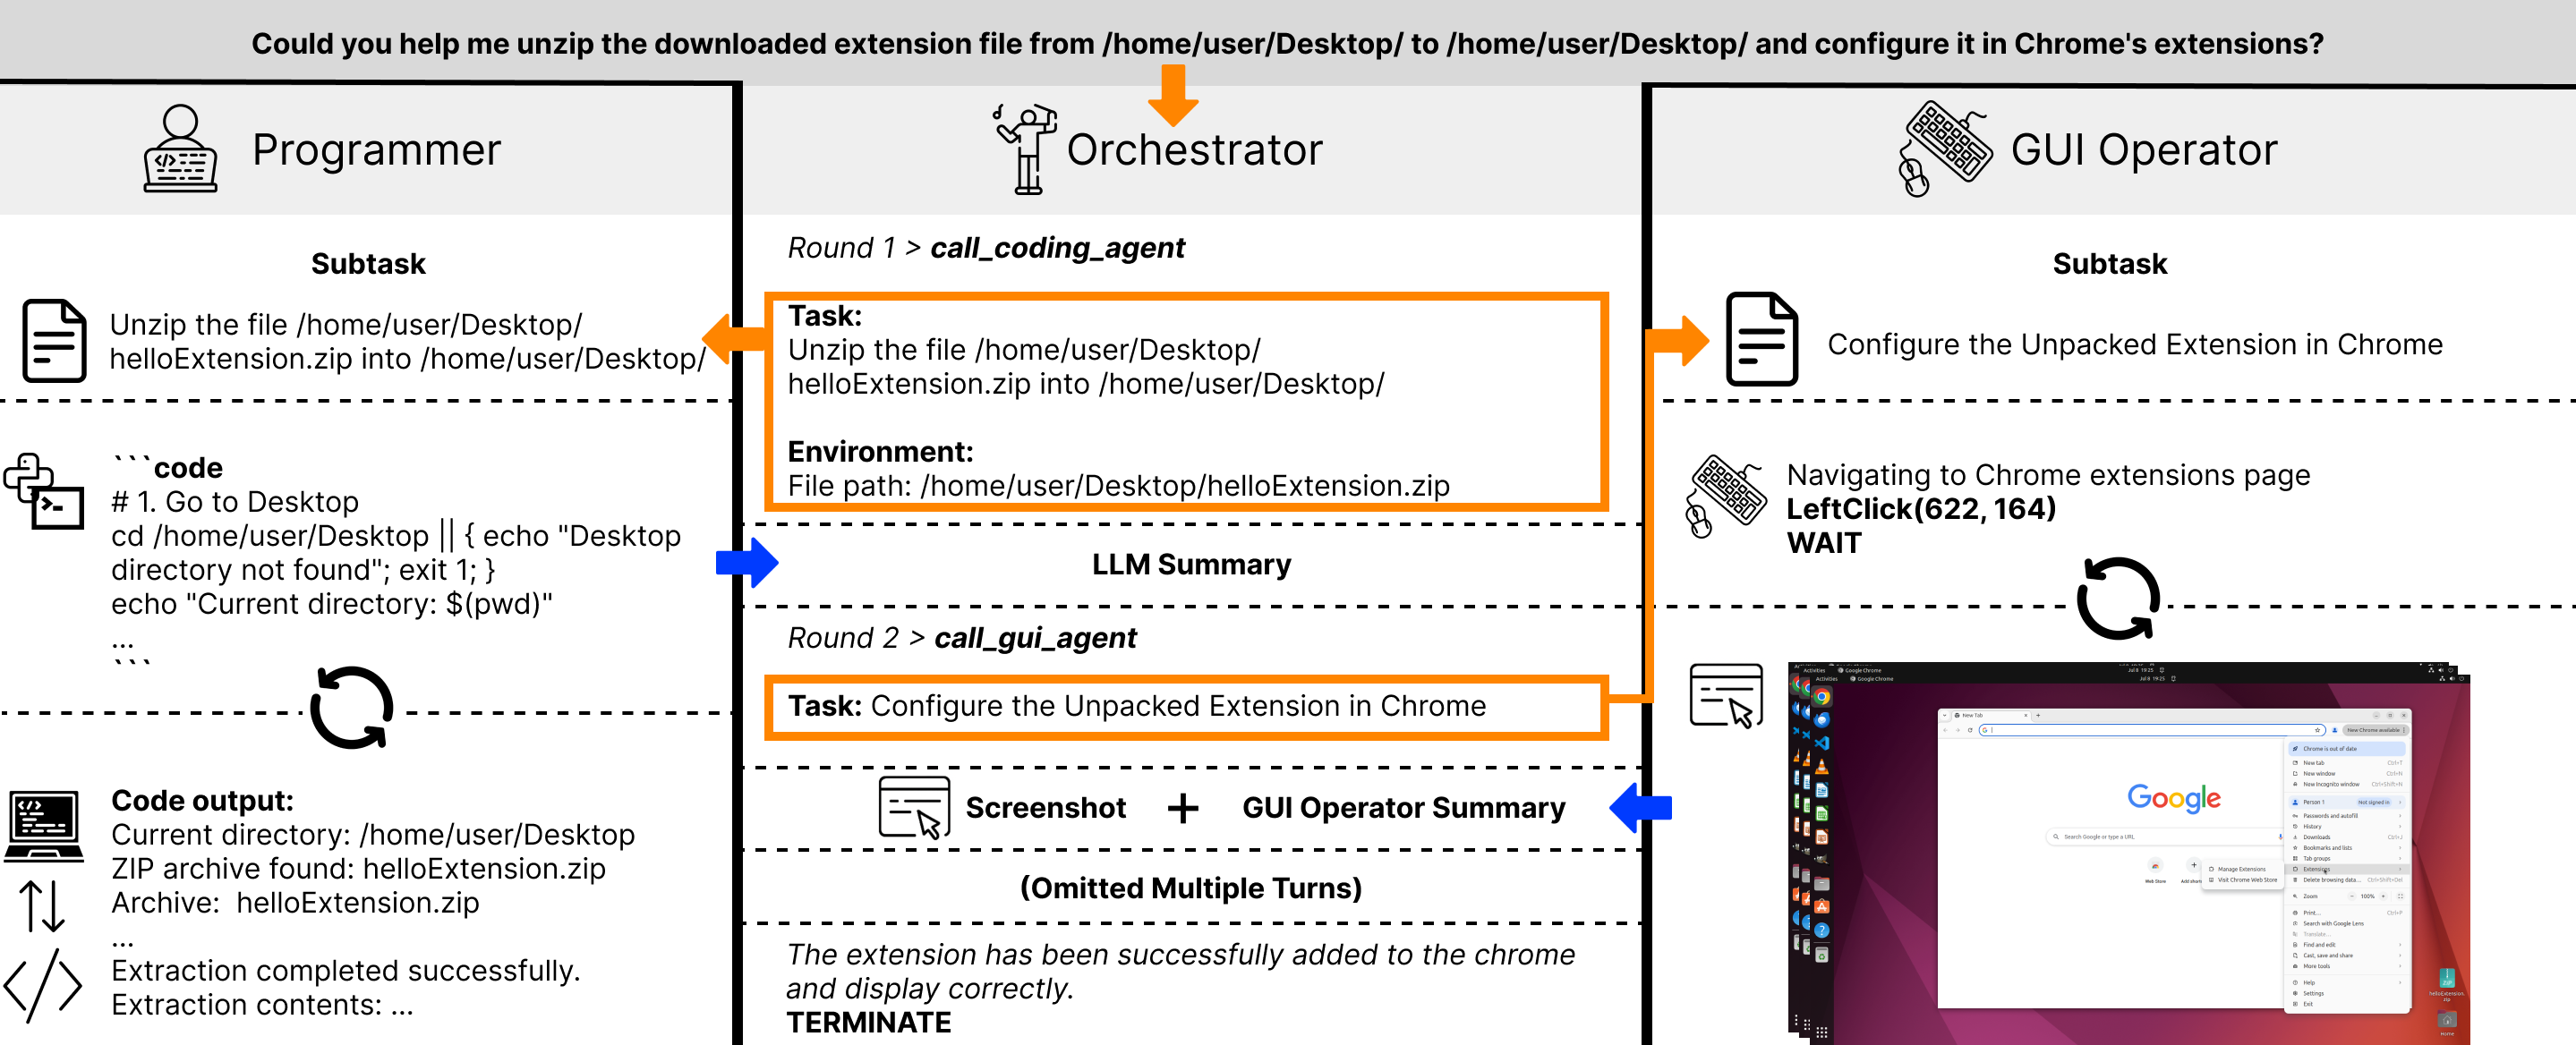
\includegraphics[width=\linewidth]{figures/workflow.png}
    \caption{\ours 工作流示意图。对于给定用户任务，编排器可以选择调用编程员或 GUI 操作员解决子任务。编程员通过编码与操作系统交互，GUI 操作员则通过 GUI 操作与系统交互。}
    \label{fig:workflow}
\end{figure}
\ours 所实现的层次化策略，需要一个结构化工作流和记忆系统来管理智能体之间的信息流。该设计确保每个智能体都拥有必要上下文，同时不会被任务其他部分的无关细节淹没。整体工作流如\autoref{fig:workflow}所示。

\paragraph{工作流。} 工作流开始时，充当元策略 $\pi_{\text{Orch}}$ 的编排器将子任务委派给合适的执行智能体，即编程员或 GUI 操作员。选中的智能体随后进入自己的多轮交互循环以解决子任务，并产生记录其动作与环境响应的详细对话历史。子任务完成后，专用摘要模型处理这段详细历史，把整个交互压缩为简洁摘要，其中涵盖关键动作和最终结果。该摘要连同表示环境新状态的最终屏幕截图一起返回编排器。这一交接机制为编排器提供了对总体任务历史 $H_t$ 的精炼高层更新。

\paragraph{面向任务分解的记忆设计。}
\ours 采用层次化且彼此隔离的记忆结构：
\begin{itemize}[leftmargin=0.3cm, itemindent=0cm]
    \item \textbf{编排器记忆：}编排器维护长期主记忆，对应问题定义中的历史上下文 $H_t$。它包含初始用户目标 $G$，以及每个子任务完成后从执行智能体接收的摘要与屏幕截图序列。汇总后的历史为所有高层规划决策提供上下文。
    \item \textbf{执行器记忆：}编程员和 GUI 操作员各自维护短期工作记忆，只在其所负责子任务持续期间保持活动。该记忆包含它们与操作系统多轮交互的“实例对话历史”。
\end{itemize}
为保证模块化和专注性，这些记忆彼此隔离；各智能体不会直接共享对话历史。此外，一旦执行器完成子任务并向编排器汇报，其工作记忆便会被清空。这种重置机制十分关键，因为它使执行智能体能够完全专注于新收到子任务的上下文，不受先前无关交互影响。


\section{实验}
\subsection{基准数据集}
我们在 OSWorld~\citep{xie2024osworldbenchmarkingmultimodalagents} 和 WindowsAgentArena~\citep{bonatti2024windowsagentarenaevaluating} 上评估 \ours。二者都是可扩展的真实计算机测试平台，通过像素流和操作系统 Shell 接口向智能体开放 Windows 或 Ubuntu 操作系统。OSWorld 包含 369 个任务，WindowsAgentArena 包含 154 个任务。这些任务覆盖常用生产力工具、集成开发环境、浏览器、文件管理器和多应用工作流，因而会同时考验智能体在异构 GUI 环境中的视觉语言定位与长时程规划能力。

\subsection{基线}
我们将 \ours 与两类计算机使用智能体进行比较：端到端模型和智能体方法。这些基线代表了基于 GUI 的任务自动化前沿。
\paragraph{端到端模型。}
端到端模型以用户指令和操作系统屏幕截图为输入，不使用任何智能体工作流，仅通过模型推理输出相应动作。\textit{OpenAI o3}~\citep{openAI_o3_o4_mini} 是 OpenAI 的前沿推理模型，擅长多步问题求解以及多用途、上下文感知的辅助。\textit{OpenAI CUA 4o}~\citep{cua2025} 运用视觉和推理同图形用户界面交互，控制鼠标和键盘执行任务；Operator、ChatGPT agent 等服务背后使用了这项技术。\textit{UI-TARS}~\citep{qin2025ui} 提出完全端到端、仅依赖屏幕截图的原生 GUI 智能体模型，在单一模型中统一感知、推理、记忆与动作。\textit{OpenCUA（32B）}~\citep{wang2025opencua} 则提出完全开源的框架，包含可扩展数据收集工具、首个大规模跨操作系统计算机使用任务数据集、反思式思维链推理流水线，以及强大的视觉语言智能体模型。

\paragraph{智能体方法。}
智能体方法包括规划器--定位器、规划器--多定位器等不同结构的单智能体与多智能体系统。这些基线主要通过增强语言模型的底层定位能力来改善计算机操作表现。\textit{Jedi-7B w/ o3}~\citep{xie2025scaling}：本文中的 Jedi 指在 Jedi 数据集上训练的 Qwen2.5-VL。其作者将 Jedi 接入智能体栈，把高层计划转化为像素级精确的 GUI 动作，并在 OSWorld、WindowsAgentArena 和多个定位基准上取得大幅提升。\textit{GTA-1 w/ o3}~\citep{yang2025gta1guitesttimescaling}：GUI 测试时扩展智能体 GTA-1 面向高分辨率界面中的规划歧义和动作定位难题；它采用“测试时扩展”策略，生成多个可能动作，再用裁判模型选出最优动作，并使用 GRPO 训练强定位器。\textit{Agent S2.5 w/ o3}~\citep{agashe2025agent}：Agent S2.5 是组合式规划器--多定位器框架。规划器生成高层子目标，多个定位器执行这些目标，并通过定位专家混合机制把 GUI 元素定位委派给视觉、文本和结构专家；两个层级在每个子目标之后都会主动重新规划，以适应不断变化的屏幕。

除上述强基线外，我们还在 WindowsAgentArena 上加入 Agent S~\citep{agashe2024agent} 和 NAVI~\citep{bonatti2024windowsagentarenaevaluating} 作为基线。

\subsection{实现细节}
\noindent\textbf{环境。} 我们在 Linux 上测试 \ours，并扩展了 OSWorld 的 RESTful 服务器。具体而言，我们实现了一个远程代码解释器，它可以接收较长的 Python 和 Bash 脚本，并把执行结果返回给发送方。另一方面，对于每个任务，OSWorld 都会建立初始状态，例如打开一组应用或特定网站，或者把指定文件下载到指定位置。初始状态就绪后，我们截取屏幕截图，并将其与用户任务一起作为 \ours 和各基线的初始输入。

\noindent\textbf{\ours 设置。} 我们使用 AG2~\citep{wu2023autogenenablingnextgenllm} 实现 \ours。其中，编排器采用 OpenAI o3，编程员采用 OpenAI o4-mini。GUI 操作员的骨干模型为 OpenAI computer-use-preview，这是一种由 OpenAI 针对计算机使用微调的视觉语言动作模型。我们还使用 o4-mini 作为摘要器，对编程员与编排器之间的对话历史进行总结。编程员的最大轮数 $I$ 设为 20，GUI 操作员的最大步数 $K$ 设为 25，编排器的最大轮数 $J$ 设为 15。因此，\ours 的系统交互次数（即步数）上限为 375；但如\autoref{fig:error_rate}所示，所有样例都会在 150 步之前提前停止。更多细节见\autoref{apdx:repduction-statement}。

\noindent\textbf{评估协议。}
我们使用 OSWorld 和 WindowsAgentArena 提供的基于规则的评估器评估方法。每个评估器在内部都表示为一个布尔表达式，由基准作者手工设计的 134 个基于实际执行的原子评估器构成。对于给定任务，基准使用逻辑 AND/OR 运算符组合这些原子条件；例如，“通过”可能要求（文件已导出 AND MD5 匹配）AND（邮件已发送 == True）。


\subsection{结果}

\begin{table}[t]
\centering
\caption{\label{tab:osworld_comparison}OSWorld~\citep{xie2024osworldbenchmarkingmultimodalagents} 已验证基准上最先进方法的比较。结果按步数预算分组。\textbf{办公}任务来自 LibreOffice Calc、LibreOffice Impress 和 LibreOffice Writer；\textbf{日常}任务来自 Chrome、Thunderbird 和 VLC；\textbf{专业}任务来自 GIMP 和 VSCode。各类任务均以成功率（\%）为指标；每个步数预算内的最佳结果用\textbf{粗体}标出，跨全部步数预算的最佳结果用\textbf{\best{带下划线的粗体}}标出。}
\renewcommand{\arraystretch}{1.2}
\resizebox{\textwidth}{!}{%
\begin{tabular}{lccccccccccc}
\toprule
\textbf{智能体模型}       & \multicolumn{3}{c}{\textbf{办公（104 项）}} & \multicolumn{3}{c}{\textbf{日常（78 项）}} & \multicolumn{2}{c}{\textbf{专业（48 项）}} & \textbf{操作系统（24 项）}    & \textbf{多应用（101 项）} & \multicolumn{1}{c}{\textbf{平均}} \\ \rowcolor{gray!15}
\multicolumn{12}{c}{\textit{15 步}}                                                                                                                                                                                                   \\
OpenAI o3                  & \multicolumn{3}{c}{1.45}            & \multicolumn{3}{c}{8.02}           & \multicolumn{2}{c}{12.29}                 & 37.50          & 11.82                  & 9.09                              \\
UI-TARS-1.5 (7B)             & \multicolumn{3}{c}{27.19}           & \multicolumn{3}{c}{27.99}          & \multicolumn{2}{c}{61.45}                 & 34.78          & 5.38                  & 25.76                            \\
OpenAI CUA 4o              & \multicolumn{3}{c}{22.17}           & \multicolumn{3}{c}{37.65}          & \multicolumn{2}{c}{41.22}                 & 45.83          & 10.75                  & 26.01                             \\
OpenCUA              & \multicolumn{3}{c}{26.69}           & \multicolumn{3}{c}{33.25}          & \multicolumn{2}{c}{51.57}                 & 43.48          & 10.41                  & 28.12                             \\
Agent S2.5 w/ o3           & \multicolumn{3}{c}{42.85}           & \multicolumn{3}{c}{44.61}          & \multicolumn{2}{c}{57.10}                 & \textbf{70.83}          & 17.82                  & 38.98                             \\
Jedi-7B w/ o3              & \multicolumn{3}{c}{45.84}           & \multicolumn{3}{c}{\textbf{57.49}} & \multicolumn{2}{c}{\textbf{60.95}}        & 50.00          & 20.43                  & \textbf{42.37}                    \\\rowcolor[HTML]{DBFCDA}
\ours                    & \multicolumn{3}{c}{\textbf{47.18}}  & \multicolumn{3}{c}{42.30}          & \multicolumn{2}{c}{47.74}                 & 66.67 & \textbf{23.82}         & 39.81                             \\\rowcolor{gray!15}
\multicolumn{12}{c}{\textit{50 步}}                                                                                                                                                                                                   \\
OpenAI o3                  & \multicolumn{3}{c}{11.50}           & \multicolumn{3}{c}{19.78}          & \multicolumn{2}{c}{30.10}                 & 37.50          & 11.82                  & 17.17                             \\
UI-TARS-1.5 (7B)             & \multicolumn{3}{c}{26.51}           & \multicolumn{3}{c}{31.41}          & \multicolumn{2}{c}{48.91}                 & 25.00          & 9.77                  & 25.08                            \\
OpenAI CUA 4o              & \multicolumn{3}{c}{23.56}           & \multicolumn{3}{c}{38.43}          & \multicolumn{2}{c}{52.09}                 & 70.83          & 15.86                  & 31.19                             \\
OpenCUA              & \multicolumn{3}{c}{30.06}           & \multicolumn{3}{c}{42.31}          & \multicolumn{2}{c}{58.28}                 & 47.83          & 16.79                  & 33.76                             \\
GTA-1-7B w/ o3             & \multicolumn{3}{c}{48.58}           & \multicolumn{3}{c}{52.31}          & \multicolumn{2}{c}{\textbf{\best{77.84}}}        & 58.33          & 37.05                  & 48.59                             \\
Jedi-7B w/ o3              & \multicolumn{3}{c}{50.10}           & \multicolumn{3}{c}{\textbf{65.25}}          & \multicolumn{2}{c}{68.65}                 & 54.17          & 34.97                  & 50.65                             \\
Agent S2.5 w/ o3           & \multicolumn{3}{c}{52.81}           & \multicolumn{3}{c}{55.80}          & \multicolumn{2}{c}{75.42}                 & \textbf{\best{75.00}} & 39.53                  & 54.21                             \\\rowcolor[HTML]{DBFCDA}
\ours                    & \multicolumn{3}{c}{\textbf{62.91}}  & \multicolumn{3}{c}{59.43} & \multicolumn{2}{c}{69.89}                 & 70.83          & \textbf{42.37}         & \textbf{56.38}                    \\\rowcolor{gray!15}
\multicolumn{12}{c}{\textit{100 步}}                                                                                                                                                                                                  \\
OpenAI o3                  & \multicolumn{3}{c}{17.23}           & \multicolumn{3}{c}{26.29}          & \multicolumn{2}{c}{38.79}                 & 62.50          & 16.53                  & 23.00                             \\
UI-TARS-1.5 (7B)             & \multicolumn{3}{c}{25.01}           & \multicolumn{3}{c}{31.07}          & \multicolumn{2}{c}{46.99}                 & 29.17          & 8.80                  & 25.41                            \\
OpenAI CUA 4o              & \multicolumn{3}{c}{25.04}           & \multicolumn{3}{c}{39.19}          & \multicolumn{2}{c}{55.43}                 & 58.33          & 18.48                  & 31.38                             \\
OpenCUA              & \multicolumn{3}{c}{30.06}           & \multicolumn{3}{c}{38.89}          & \multicolumn{2}{c}{60.70}                 & 52.17          & 18.10                  & 33.84                             \\
Jedi-7B w/ o3              & \multicolumn{3}{c}{47.89}           & \multicolumn{3}{c}{64.37}          & \multicolumn{2}{c}{\textbf{75.92}}        & 50.00          & 35.27                  & 50.98                             \\
GTA-1-7B w/ o3             & \multicolumn{3}{c}{55.68}           & \multicolumn{3}{c}{\textbf{64.74}} & \multicolumn{2}{c}{61.20}                 & 62.50          & 38.34                  & 53.07                             \\
Agent S2.5 w/ o3           & \multicolumn{3}{c}{54.23}           & \multicolumn{3}{c}{55.80}          & \multicolumn{2}{c}{75.42}                 & \textbf{\best{75.00}}          & 44.06                  & 55.98                             \\\rowcolor[HTML]{DBFCDA}
\ours                    & \multicolumn{3}{c}{\textbf{\best{64.80}}}  & \multicolumn{3}{c}{61.60}          & \multicolumn{2}{c}{71.82}                 & \textbf{\best{75.00}} & \textbf{\best{47.87}}         & \textbf{59.93}                             \\ \rowcolor{gray!15}
\multicolumn{12}{c}{\textit{150 步}}                                                                                                                                                                                                 \\\rowcolor[HTML]{DBFCDA}
\ours                    & \multicolumn{3}{c}{\textbf{\best{64.80}}}           & \multicolumn{3}{c}{\best{\textbf{66.51}}}          & \multicolumn{2}{c}{71.82}                 & \textbf{\best{75.00}}          & \textbf{\best{47.87}}                  & \textbf{\best{60.76}}                             \\ \bottomrule
\end{tabular}%
}
\end{table}

\begin{table}[t]
\centering
\caption{\label{tab:waa_comparison}WindowsAgentArena~\citep{bonatti2024windowsagentarenaevaluating} 上最先进方法的比较。结果按步数预算分组。\textbf{办公}任务来自 LibreOffice Calc 和 LibreOffice Writer；\textbf{网页}任务来自 Chrome 与 Microsoft Edge；\textbf{Windows 系统}任务来自“设置”和文件资源管理器；\textbf{Windows 工具}任务来自时钟、Windows 计算器、记事本和 Microsoft Paint。各类任务均以成功率（\%）为指标，最佳结果用\textbf{粗体}标出。}
\resizebox{\textwidth}{!}{%
\begin{tabular}{lccccccc}
\toprule
\textbf{方法}              & \textbf{办公（43 项）} & \textbf{网页（30 项）}  & \textbf{Windows 系统（24 项）} & \textbf{VSCode（24 项）} & \textbf{VLC（21 项）} & \textbf{Windows 工具（12 项）} & \textbf{平均} \\ \midrule
Agent S             & 0.0    & 13.3 & 45.8           & 29.2   & 19.1           & 22.2          & 18.2    \\
NAVI                & 0.0    & 27.3 & 33.3           & 27.3   & 30.3           & 8.3           & 19.5    \\
Agent S2            & 7.0    & 16.4 & 54.2           & \textbf{62.5}   & 28.6           & 33.3          & 29.8    \\ \midrule
\rowcolor[HTML]{DBFCDA}
\ours (15 steps)  & 8.7    & 3.3  & 50.0           & 29.2   & 23.8           & 44.4          & 21.4    \\
\rowcolor[HTML]{DBFCDA}
\ours (50 steps)  & 26.1   & 33.3 & 75.0           & 54.2   & 42.4           & 55.6          & 43.5    \\
\rowcolor[HTML]{DBFCDA}
\ours (100 steps) & \textbf{30.4}   & \textbf{50.0} & \textbf{83.3}           & \textbf{62.5}   & \textbf{47.2}           & \textbf{77.7}          & \textbf{52.5}    \\ \bottomrule
\end{tabular}%
}
\end{table}

\autoref{tab:osworld_comparison}和\autoref{tab:waa_comparison}所列实验结果明确表明，\ours 在两个具有挑战性的真实计算机操作基准上均达到新的最先进水平。这些发现验证了我们的核心假设：在传统 GUI 操作之外整合程序化动作，可以形成更稳健、更高效且更具泛化能力的计算机自动化范式。

\paragraph{OSWorld 上的表现。}
在综合性 OSWorld 基准（\autoref{tab:osworld_comparison}）上，\ours 展现出更优的性能与效率。在 150 步限制内，它最终取得 60.76\% 的成功率，显著领先 Agent S2.5 w/ o3（55.98\%）和 GTA-1 w/ o3（53.07\%）等当前最强智能体框架。混合架构的优势不仅体现在峰值表现，也体现在面对不同任务复杂度时的一致性：在 100 步时，\ours 已以 59.93\% 的成功率领先，并超过所有其他基线的最终成绩。
在程序化控制最有效的类别中，本方法优势尤其明显。对于需要复杂数据或文件系统交互的任务，\ours 在办公、操作系统和多应用类别上分别达到 64.80\%、75.00\% 和 47.87\%。这些领域历来是纯 GUI 智能体较为脆弱之处；上述出色表现凸显了把后端操作委派给编程员智能体的有效性，因为它可以针对电子表格、文件操作和跨应用数据流执行精确可靠的脚本。

\paragraph{WindowsAgentArena 上的表现。} 我们进一步在 WindowsAgentArena 基准（\autoref{tab:waa_comparison}）上评估 \ours。结果显示，该框架能够把能力成功迁移到另一种操作系统，并再次以较大优势达到最先进水平。\ours 的总体成功率为 52.5\%，相较 Agent S2（29.8\%）和 NAVI（19.5\%）等先前领先方法有显著提升。WindowsAgentArena 上的分类结果进一步支持了我们的核心主张：\ours 在系统级和工具类任务上优势突出，Windows 系统与 Windows 工具类别分别达到 83.3\% 和 77.7\%。这些类别涉及文件资源管理器、系统设置和其他原生工具，非常适合编程员执行基于脚本的动作。此外，随着步数预算增加，\ours 的性能展现出清晰有效的扩展趋势：从 15 步时的 21.4\% 上升至 100 步时的 52.5\%，说明它具备解决更复杂长时程问题的能力。

综上，\ours 在两个不同且富有挑战性的基准上都稳定达到最先进水平，这证明其混合智能体架构，是朝着构建能力更强、可靠性更高的通用计算机使用自主智能体迈出的重要一步。


\subsection{讨论}
\begin{figure}[t!]
  \centering
  \begin{subfigure}[t]{0.48\linewidth}
    \centering
    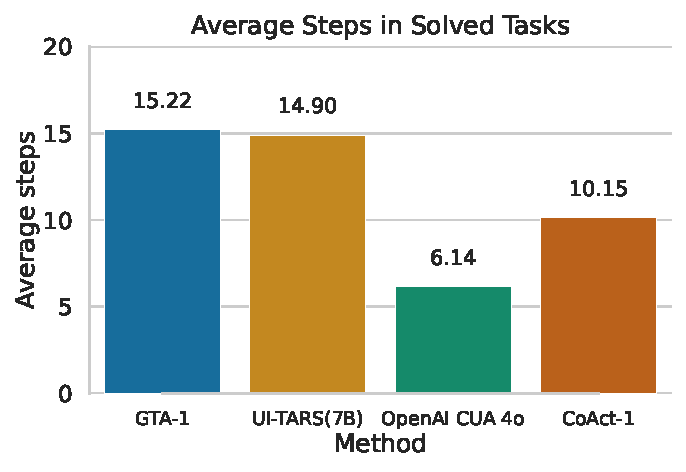
\includegraphics[width=\linewidth]{figures/avg_steps.pdf}
    \caption{在 100 步预算下，每个成功任务的平均步数；\ours 的效率显著高于 GTA-1 等其他最先进智能体框架。}
    \label{fig:avg_steps}
  \end{subfigure}
  \hfill
  \begin{subfigure}[t]{0.48\linewidth}
    \centering
    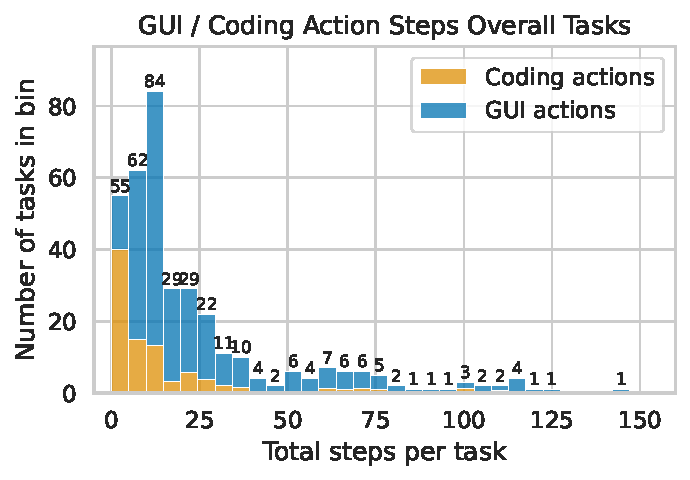
\includegraphics[width=\linewidth]{figures/gui_cod_actions.pdf}
    \caption{按总步数划分的任务分布，同时展示编码动作与 GUI 动作的比例，表明编码有助于减少总动作步数。}
    \label{fig:gui_cod_actions}
  \end{subfigure}%
    \hfill
  \begin{subfigure}[t]{0.48\linewidth}
    \centering
    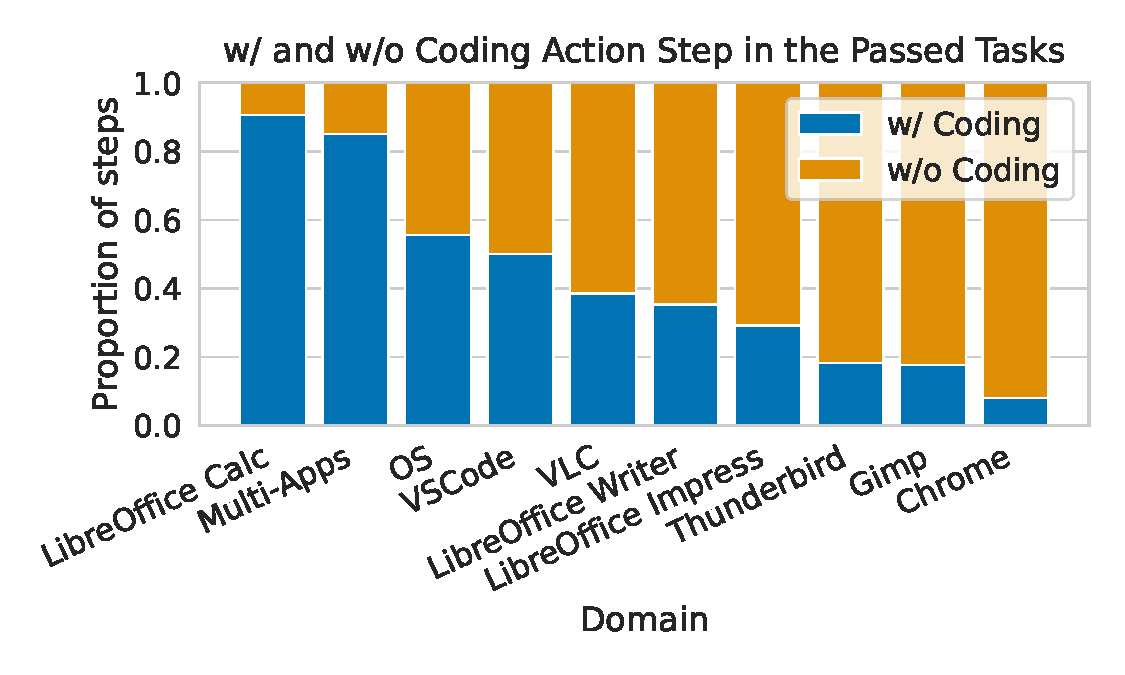
\includegraphics[width=\linewidth]{figures/coding_vs_non_coding.pdf}
    \caption{按应用领域划分的成功任务；编码动作最常用于 LibreOffice Calc、多应用和直接操作系统交互等复杂领域。}
    \label{fig:coding_ratio}
  \end{subfigure}%
  \hfill
  \begin{subfigure}[t]{0.48\linewidth}
    \centering
    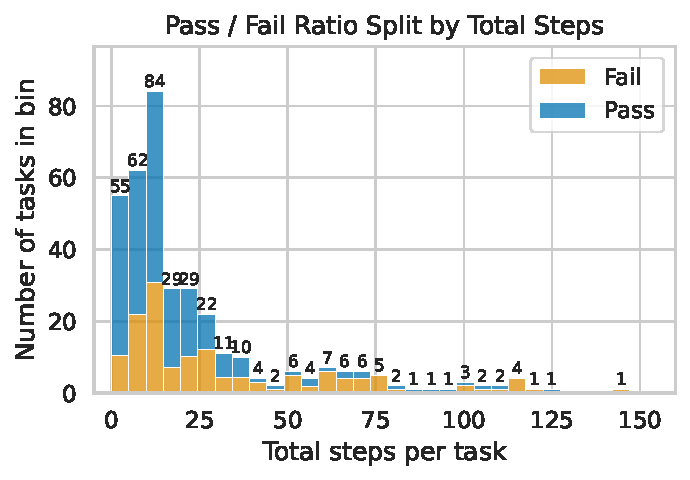
\includegraphics[width=\linewidth]{figures/error_rate.pdf}
    \caption{按总步数划分的通过/失败比例，表明失败率与所需动作数呈正相关。}
    \label{fig:error_rate}
  \end{subfigure}%
  \caption{\ours 的效率与动作步模态分析。}
  \label{fig:agent_metrics}
\end{figure}
\paragraph{效率分析。}
\autoref{fig:agent_metrics}所示的 \ours 操作效率分析表明，我们的混合方法明显比领先的纯 GUI 智能体更高效，而这种效率是其成功率提高的关键因素。如\autoref{fig:avg_steps}所示，\ours 解决任务平均需要 10.15 步，显著优于 GTA-1 的 15.22 步和 UI-TARS 的 14.90 步。OpenAI CUA 4o 的平均步数虽更少（6.14），但总体成功率远低于 \ours（在 100 步预算下分别为 31.40\% 与 59.93\%），这说明 \ours 的效率同时伴随着更强的有效性。效率来源在于对编码动作的策略性运用。\autoref{fig:gui_cod_actions}显示，编码动作有助于使每个任务的总步数保持在较低水平，而这对稳健表现至关重要。\autoref{fig:coding_ratio}表明，在 LibreOffice Calc、多应用和直接操作系统交互等复杂领域，编码尤其有益；其中很大比例的任务由代码解决。一个脚本可以替代漫长且易错的 GUI 点击序列，从而简化工作流。\autoref{fig:error_rate}还揭示出清晰趋势：需要更多动作的任务更容易失败。通过减少总步数，混合方法既能加快任务完成，也能减少出现错误的机会。动态选择最合适动作——直接编码命令或 GUI 交互——是 \ours 提升效率和可靠性的根本所在。


\paragraph{使用不同骨干模型的 \ours。}
\begin{table}[t]
\centering
\caption{\label{tab:model-abla}\ours 中各参与智能体采用不同骨干模型时的性能。更强的编排器能够显著改善 OSWorld 上的表现。}
\renewcommand{\arraystretch}{1.2}
\resizebox{0.6\textwidth}{!}{%
\begin{tabular}{lllc}
\hline
\textbf{GUI 操作员} & \textbf{编排器} & \textbf{编程员} & \textbf{性能（\%）} \\ \hline
\multirow{3}{*}{OpenAI CUA 4o} & o4-mini & o4-mini & 43.43 \\
                               & o3      & o3      & 58.72 \\
                               & o3      & o4-mini & 60.76 \\ \hline
\end{tabular}%
}
\end{table}
我们在 OSWorld 基准上研究了为 \ours 各智能体组件选择不同骨干模型的影响，结果见表~\ref{tab:model-abla}。分析显示，系统总体性能对编排器和编程员所用模型的推理与指令遵循能力高度敏感。当编排器和编程员都使用 o4-mini、GUI 操作员使用 OpenAI CUA 4o 时，系统性能为 43.43\%。编排器和编程员都改用更强的 o3 后，性能显著提升至 58.72\%，说明复杂高层规划器与有能力的代码生成器对系统成功至关重要。异构配置取得最高的 60.76\%：编排器使用 o3、编程员使用 o4-mini，GUI 操作员仍使用 OpenAI CUA 4o。这一配置显示出一种较优平衡——利用 o3 的强推理能力完成任务分解与委派，同时受益于 o4-mini 面向代码生成的专门能力。结果表明，增强编排器和编程员能力能够带来最显著的性能收益；这既验证了模块化设计，也展示了把强模型策略性分配给高推理需求角色的价值。


\paragraph{纯 GUI 动作与纯编码动作。}
\begin{table}[t]
\centering
\caption{\label{tab:module-abla}\ours 组件性能的消融研究。我们比较完整混合系统、仅使用编程员（纯编码）的智能体，以及仅使用 GUI 操作员（纯 GUI）的智能体。整合后的 \ours 显著优于任一单模态智能体，说明混合方法有效。}
\resizebox{\textwidth}{!}{%
\begin{tabular}{ccccccccc}
\toprule
\multicolumn{2}{c}{\textbf{\ours}}     & \multirow{2}{*}{\textbf{办公}} & \multirow{2}{*}{\textbf{日常}} & \multirow{2}{*}{\textbf{专业}} & \multirow{2}{*}{\textbf{操作系统}} & \multirow{2}{*}{\textbf{多应用}} & \multirow{2}{*}{\textbf{平均}} & \multirow{2}{*}{\textbf{平均步数}} \\ \cmidrule(lr){1-2}
含编程员 & 含 GUI 操作员 &                         &                        &                               &                     &                                &                       &                             \\ \midrule
$\checkmark$             &                 & 40.88                   & 16.17                  & 53.06                         & 62.50      & 29.63                          & 35.73                 & \textbf{1.14}               \\
              & $\checkmark$                 & 43.50                   & 58.80                  & 69.38                         & \textbf{79.16}               & 35.68                          & 50.68                 & 11.20                       \\
$\checkmark$               & $\checkmark$                 & \textbf{64.80}          & \textbf{66.51}         & \textbf{71.82}                & 75.00               & \textbf{47.87}                 & \textbf{60.76}        & 10.15                       \\ \bottomrule
\end{tabular}%
}
\end{table}
为分离各智能体模态并验证混合设计，我们开展消融实验，将完整 \ours 系统与只能使用单一动作类型的智能体进行比较。\autoref{tab:module-abla}显示组合方法更优。仅含编程员的智能体（纯编码）取得 35.73\% 的成功率，说明许多任务除了脚本之外仍需要 GUI 交互。该智能体效率很高，每个成功任务平均仅需 1.14 步，印证了程序化动作的直接性。仅含 GUI 操作员的智能体（纯 GUI）可以处理更多任务类型，成功率更高，达到 50.68\%，但每个任务需要 11.20 步。整合两种模态的完整 \ours 模型取得 60.76\% 的成功率，平均使用 10.15 步，体现了该架构的协同效应：编排器在后端任务中发挥编程员的高效率，又在视觉导航中利用 GUI 操作员的通用性，从而构成稳健系统。


% \paragraph{Scaling steps for computer-using agent}


\section{结论}
本文提出 \ours，这是一种新型多智能体系统，旨在解决完全依赖 GUI 操作的智能体所固有的低效与脆弱性。该系统包含一个编排器，能够把子任务动态委派给 GUI 操作员或编程员。我们在 OSWorld 和 WindowsAgentArena 基准上进行了广泛评估，验证了这种方法的有效性。\ours 在 OSWorld 和 WindowsAgentArena 上分别取得 60.76\% 和 52.5\% 的成功率，均达到新的最先进水平，并显著优于先前领先方法。在涉及操作系统级交互、多应用工作流，以及编程员智能体能够利用直接程序化执行的其他任务类别中，性能提升尤其明显。

\bibliography{main}
\bibliographystyle{iclr2026_conference}

\appendix
\section{大语言模型使用声明}
我们使用大语言模型（OpenAI 的 o3 和 GPT-5）作为通用写作辅助工具，其作用仅限于句子与段落层面的润色，包括改善清晰度、语法和行文流畅性。全部研究想法、分析、结果和结论均由作者提出。模型没有生成新内容、开展文献综述，也未参与论文概念框架的构建。

\section{伦理声明}
本研究旨在推动计算机自动化服务于有益且富有生产力的用途，但我们也承认其潜在的军民两用属性及相关风险。

\noindent\textbf{安全与滥用：}能够执行代码（Python 或 Bash）并操作 GUI 的智能体，若缺乏适当约束，可能被用于恶意活动。为在研究过程中缓解这一风险，全部实验均在安全、隔离且虚拟化的基准环境（OSWorld 和 WindowsAgentArena）中开展。这确保智能体动作被限制在沙箱内，不会影响现实系统或数据。我们主张，未来若在真实环境中部署此类智能体，必须纳入稳健的安全协议、严格的权限控制，以及阻止有害代码执行的机制。

\noindent\textbf{数据隐私：}智能体通过屏幕截图观察屏幕，而现实场景中的截图可能包含敏感信息或个人信息。本文仅使用基准任务中提供的数据，不涉及真实用户数据。任何未来应用都必须实施严格的数据处理政策和隐私保护技术，以保护用户机密信息。


\section{可复现性声明}
\label{apdx:repduction-statement}
复现 \ours 需要准确使用特定 OpenAI 模型和提示词。请仔细核对以下细节，以确保正确复现本文工作表现。

\subsection{模型使用与环境设置}
\paragraph{模型使用。}
 本文使用 \texttt{o3-2025-04-16} 作为编排器，\texttt{o4-mini-2025-04-16} 作为编程员，\texttt{computer-use-preview-2025-03-11} 作为 GUI 操作员。只要满足以下要求，\ours 也可以采用任意开源模型：
\begin{itemize}[leftmargin=0.3cm, itemindent=0.3cm]
    \item \textbf{编排器：}编排器需要多模态输入（图像和文本），以处理操作系统的全部屏幕截图并进行规划；它还需要较强的跨模态推理能力（见\autoref{tab:model-abla}，推理能力会显著影响最终表现）。
    \item \textbf{GUI 操作员：}GUI 操作员可以替换为 UI-TARS~\citep{qin2025ui}、OpenCUA~\citep{wang2025opencua} 等任意开源视觉语言动作模型（VLA），也可以替换为 GTA-1~\citep{yang2025gta1guitesttimescaling}、Agent S2~\citep{agashe2025agent} 等规划器--定位器方法。\ours 要求 GUI 操作员具备两类能力：（1）定位任务之外的指令遵循能力，例如判断何时终止；（2）计算机使用能力，包括\textit{点击}、\textit{拖拽}、\textit{输入}和\textit{快捷键}。遗憾的是，本研究没有获得足够 GPU 资源来测试这些模型在 \ours 中的表现；若把 GUI 操作员替换为更强模型，预计平均步数会下降，性能会提升。
    \item \textbf{编程员：}用于编程员的语言模型应具备较强的 Python 和 Bash（Windows 中为 PowerShell）编写能力，以解决计算问题。需要注意的是，我们没有向编程员提供任何 API 或 SDK；不过，可以把这作为本方法的扩展，以改善 Chrome、Thunderbird 等特定应用任务上的表现。
\end{itemize}

\paragraph{环境。}
评估计算机使用智能体时，操作系统环境本身也是一项重大挑战。为复现实验结果，编排器收到的所有输入截图都应准确反映初始化良好的系统状态。因此，我们建议在虚拟机启动后等待 60 秒，再截取操作系统屏幕，以确保截图包含编排器进行规划所需的全部信息。

\subsection{\ours 的提示词设计}
任何现代大语言模型智能体系统的性能，都可能受到提示词或模板设计的显著影响~\citep{he2024doespromptformattingimpact}。在 \ours 中，除思维链、验证等通用行为规则外，我们还针对模型局限制定规则。具体而言，我们观察到 GUI 操作员在自检时具有较高的幻觉率；另一方面，编程员对文件的修改不会直接反映在操作系统屏幕上，因此编排器无法捕捉变化并规划下一步。提示词设计通过允许编排器独立检查结果，并重新加载编程员修改过的文件来缓解这些局限。OSWorld 与 WindowsAgentArena 所用提示词见\autoref{tab:prompt-orchestrator-1}、\autoref{tab:prompt-orchestrator-2}、\autoref{tab:prompt-gui-operator}、\autoref{tab:prompt-programmer}和\autoref{tab:prompt-llm-summarizer}。为保持实验材料逐字可复现，以下提示词框保留英文原文。



\section{\ours 何时以及为何失败？对未来工作的启示}
为更好地理解 \ours 的能力与局限，本节分析评估过程中观察到的失败案例。总体而言，任务完成错误主要源自四类挑战：高层查询、歧义查询、反思错误和幻觉。

\textbf{高层查询。} 高层查询是指用户指令无法直接映射为动作序列的查询。智能体必须先推断用户的潜在意图和更广泛上下文，才能设计解决方案。
例如，一个 VSCode 任务要求智能体：“请帮我修改 VSCode 设置，使我在 VSCode 中调试时，光标保持聚焦于调试控制台，而不是自动切回编辑器。”在该场景中，编排器将任务委派给编程员。编程员尝试通过搜索“debug”“console”等关键词来查找相关设置，却未能推断调试过程与“breakpoints”有关。因此，它漏掉了正确设置项“focusEditorOnBrake”，导致任务失败。该案例揭示了智能体对查询中未明确出现的概念进行推理时所面临的局限。

\textbf{歧义查询。}
歧义查询是含糊不清，或省略了成功完成任务所需关键信息的用户请求。消除歧义往往要求智能体正确推断用户意图，其中也可能涉及安全考量。
例如，一个 VSCode 任务要求：“请帮我修改 VSCode 设置，在资源管理器视图中隐藏所有 `\_\_pycache\_\_` 文件夹。”编排器把该子任务交给编程员。编程员正确识别出需要修改设置文件，却错误地修改了工作区专用设置，而不是全局用户设置。它对查询范围的错误理解导致任务失败。这说明，当存在多个合理解释时，智能体在消解用户意图歧义方面会遇到挑战。

\textbf{反思错误。}
反思是 \ours 验证任务完成过程的关键机制。在我们的系统设计中，GUI 操作员完成任务后，只有操作系统最终状态会返回编排器。若 GUI 操作员在中间状态犯错，且后续操作遮蔽了该错误，系统最终就可能出错。例如，进行电子表格操作时，GUI 操作员可能在某个单元格（假设位于 A 行）中输错内容，随后向下滚动电子表格并停在那里。此时，本方法返回的操作系统截图不会包含 A 行中的错误值，编排器无法捕捉该错误，任务最终会因这次非预期操作而失败。

\textbf{幻觉。}
幻觉是大语言模型时代最重要的议题之一，也是导致 \ours 失败的常见原因。\ours 中的所有智能体在求解任务时都可能产生幻觉，其中编排器和 GUI 操作员的幻觉最为显著。
编排器可能给出错误计划，其中通常包含超前预测，并进一步影响 GUI 操作员和编程员。例如，编排器可能预测尚未打开网站的内容，并指示 GUI 操作员对并不存在的内容执行操作。GUI 操作员也可能在推理过程中产生幻觉，误以为已经完成被委派的任务。本文通过提示编排器更频繁地执行验证，并对 GUI 操作员与编程员的结果进行交叉验证，来缓解编排器幻觉。


\begin{table*}[h]
\begin{tcolorbox} [colback=yellow!10]
{\bf 编排器系统提示词（第 1 部分，英文原文）}

\tcblower
Today is \{today\}.\\

\#\# Your Role\\
You are responsible for completing a computer-based task, step by step, using the tools provided.\\
You are working on a \{system\_info\} system.\\
\\
\#\#\# Step-by-Step Process\\
1. \textbf{Describe the Screenshot}\\
   - Carefully review and clearly describe the screenshot's content.\\

2. \textbf{Plan the Task}\\
   - Create a detailed, step-by-step plan to solve the task.\\
   - List all user requirements, including exact file names, file paths, and any other specifics in the output (not in the thinking).\\

3. \textbf{Execute the Instructions}\\
   - Think carefully and follow the user's instructions exactly. \textbf{Do not} make any changes not requested by the user (such as renaming files or changing file content).\\
   - You \textbf{must} apply all the changes to the computer.\\
   - If the task is impossible (e.g., missing files, wrong environment), reply with \textbf{INFEASIBLE} to end the conversation.\\
   - For file operations (like modifying spreadsheets), you MUST try the Programmer (call\_programmer) first.\\
   - When the user ask you to create a new sheet in spreadsheet, always name it sequencially. For example, `Sheet1`, `Sheet2`, etc.\\

4. \textbf{Verify the Result}\\
   - \textbf{ALWAYS} check the result through the screenshot by yourself. You can let a GUI Operator to navigate to the correct location for you. After the GUI Operator complete, the screenshot will automatically be returned to you.\\
   - If you used the Programmer to modify a file, have the GUI Operator reopen the file to see the updated results.\\
   - Ensure that the result meets all user requirements. \\
   - All the things out of the user's instructions should not be changed.
\end{tcolorbox}
\caption{\label{tab:prompt-orchestrator-1}编排器系统提示词（第 1 部分，保留英文原文）。}
\end{table*}


\begin{table*}[t]
\begin{tcolorbox} [colback=yellow!10]
{\bf 编排器系统提示词（第 2 部分，英文原文）}

\tcblower
\#\# Tools You Can Use\\

\#\#\# Programmer (call\_programmer)\\
- Can run Python or Bash code to perform most file or system tasks.\\
- Needs a clear environment description and detailed task instructions.\\
- Can use any Python package you specify.\\
- After modifying a file, ALWAYS verify every change by yourself. You can let a GUI Operator to navigate to the correct location and check the result by yourself. If something is wrong, tell the Programmer to fix it.\\
Programmer will return a summary of its task solving process after completing the task. No screenshot is provided after the Programmer completes the task.\\

\#\#\# GUI Operator (call\_gui\_operator)\\
- Can interact with the GUI by clicking on a exact position, scrolling, dragging, typing, and using hotkeys.\\
- Require a detailed task description.\\
- The GUI Operator may not able to complete your task in 100\% of accuracy and often make mistakes. \\
- Have a \textbf{25-step limit}, each step is a single OS interaction (one click, one hotkey/typing action, etc.).\\
- \textbf{Do not} let the GUI Operator to do any result check. You need to do it by checking the screenshot yourself.\\
I will return a screenshot that reflect the final state of the computer after completing the task. You don't need to prompt the GUI Operator do this.\\

\textbf{Note:} Only call ONE tool (call\_programmer or call\_gui\_operator) per reply.
\end{tcolorbox}
\caption{\label{tab:prompt-orchestrator-2}编排器系统提示词（第 2 部分，保留英文原文）。}
\end{table*}


\begin{table*}[t]
\begin{tcolorbox} [colback=yellow!10]
{\bf GUI 操作员系统提示词（英文原文）}

\tcblower
\# Your role\\
You can control the computer by clicking, scrolling, dragging, and typing.
Think carefully and execute the user's step-by-step instructions.\\
\\
\# Credentials\\
The user's password is "\{CLIENT\_PASSWORD\}". Use it when a system password prompt appears.\\
\\
\# Operating rules\\
- Keep apps open at the end of the task.\\
- If the UI doesn't appear, perform a brief, deterministic retry (e.g., refocus and re-click).\\
- Do not close the window, minimize the window unless told to do so.\\
\\
\# Response protocol\\
When you think the requested task is completed or cannot be completed, reply \textbf{exactly}:\\
`TERMINATE: <1. detailed description of what you see currently. As detailed as possible. 2. What you did to complete the task or why this task cannot be completed.>`
\end{tcolorbox}
\caption{\label{tab:prompt-gui-operator}GUI 操作员系统提示词（保留英文原文）。}
\end{table*}


\begin{table*}[t]
\begin{tcolorbox} [colback=yellow!10]
{\bf 编程员系统提示词（英文原文）}

\tcblower
\# Your role\\
You are the \textbf{lead programmer}. Solve the user's task step by step using the terminal (supports Python and Bash).\\
Your username is `user`; the sudo password is `{CLIENT\_PASSWORD}`.\\
The terminal streams real-time execution output.\\

\# Coding format\\
Submit \textbf{one} fenced code block \textbf{only}, labeled with its language:\\
```bash\\
\# Your Bash script here\\
\# To use sudo, follow this pattern:\\
echo {CLIENT\_PASSWORD} | sudo -S <your commands>\\
```\\
\\
or\\
\\
```python\\
\# Your Python code here\\
\# Do not use: if \_\_name\_\_ == "\_\_main\_\_": (it will suppress output)\\
```\\
\\
\# Requirements\\
- \textbf{File names:} Do not rename files or change extensions during any file operation unless the user explicitly asks.\\
- \textbf{Code fence language:} Every fenced block must specify the language (`bash` or `python`); otherwise you will receive `unknown language unknown`.\\
- \textbf{Single block:} Wrap all code in \textbf{one} code block—do not split your submission across multiple blocks.\\
- \textbf{Spreadsheets:} When editing spreadsheets, ensure \textbf{every value} is written to the \textbf{intended cell} and \textbf{preserve the original formatting} (fonts, colors, sizes, etc.).\\
- \textbf{Dependencies:} Before importing or using a package, \textbf{check whether it is installed}; if not, install it in your submission.\\
- \textbf{Observability:} Print intermediate results to aid debugging, for example, the value you are modifying.\\
- \textbf{Final review:} Before completion, carefully inspect your result by writing test cases and confirm that nothing outside the user's instructions has changed.\\
\end{tcolorbox}
\caption{\label{tab:prompt-programmer}编程员系统提示词（保留英文原文）。}
\end{table*}


\begin{table*}[t]
\begin{tcolorbox} [colback=yellow!10]
{\bf 大语言模型摘要器提示词（英文原文）}

\tcblower
\# Programmer <-> Terminal Log Summarizer — (No Timeline/Env/Next Actions)\\
\\
\textbf{Role:} Summarize Programmer <-> Terminal logs for the \textbf{Orchestrator} so they can decide the next step immediately.  \\
\textbf{Orchestrator's task:} `\{task\}`\\
\textbf{Execution history:} `\{chat\_history\}` (prompts + outputs).\\
\\
\#\# Output\\
\\
\textbf{1) Summary (2-4 lines)} — task, what was tried, current status, why (cite key log lines / exit codes).\\
\\
\textbf{2) Commands (deduped)}\\
```bash\\
\# unique commands in run order; annotate repeats (xN)\\
```\\
\\
\textbf{3) Terminal excerpts}\\
```text\\
\# minimal evidence: head($\sim$10) … [truncated N lines] … tail($\sim$10)\\
\# always include full error traces and return codes\\
```\\
\\
\textbf{4) Artifacts / Side effects} — files/dirs changed (paths + purpose); installs/migrations.  \\
\textit{Spreadsheet:} list cells/ranges edited and confirm formatting preserved.\\
\\
\textbf{5) Errors / Blockers} — precise messages + exit codes; likely root cause from logs (no speculation).\\
\\
\textbf{6) Verification} — what checks passed (tests, file existence, row counts); what still needs verification (e.g., reopen file and confirm cell Y).\\
\\
\#\# Rules\\
- \textbf{Evidence-first}, no speculation.  \\
- \textbf{Deterministic truncation} (head/tail; note omitted lines); always include error stacks.  \\
- \textbf{Call out deltas} (what changed vs intended).  \\
- \textbf{Keep it tight}: bullets > prose.\\
\end{tcolorbox}
\caption{\label{tab:prompt-llm-summarizer}大语言模型摘要器提示词（保留英文原文）。}
\end{table*}


\end{document}
